% --------------------------------------------------------------
% This is all preamble stuff that you don't have to worry about.
% Head down to where it says "Start here"
% --------------------------------------------------------------
 
\documentclass[12pt]{article}
 
\usepackage[margin=1in]{geometry} 
\usepackage{amsmath,amsthm,amssymb}
 
\newcommand{\N}{\mathbb{N}}
\newcommand{\Z}{\mathbb{Z}}
 
\newenvironment{theorem}[2][Theorem]{\begin{trivlist}
\item[\hskip \labelsep {\bfseries #1}\hskip \labelsep {\bfseries #2.}]}{\end{trivlist}}
\newenvironment{lemma}[2][Lemma]{\begin{trivlist}
\item[\hskip \labelsep {\bfseries #1}\hskip \labelsep {\bfseries #2.}]}{\end{trivlist}}
\newenvironment{exercise}[2][Exercise]{\begin{trivlist}
\item[\hskip \labelsep {\bfseries #1}\hskip \labelsep {\bfseries #2.}]}{\end{trivlist}}
\newenvironment{problem}[2][Problem]{\begin{trivlist}
\item[\hskip \labelsep {\bfseries #1}\hskip \labelsep {\bfseries #2.}]}{\end{trivlist}}
\newenvironment{question}[2][Question]{\begin{trivlist}
\item[\hskip \labelsep {\bfseries #1}\hskip \labelsep {\bfseries #2.}]}{\end{trivlist}}
\newenvironment{corollary}[2][Corollary]{\begin{trivlist}
\item[\hskip \labelsep {\bfseries #1}\hskip \labelsep {\bfseries #2.}]}{\end{trivlist}}

\newenvironment{solution}{\begin{proof}[Solution]}{\end{proof}}

\usepackage{lipsum}
\usepackage{cleveref}
\usepackage{graphicx}
\usepackage{subcaption}
 
\begin{document}
 
% --------------------------------------------------------------
%                         Start here
% --------------------------------------------------------------
 
\title{CS324 Deep Learning\\ \textbf{Assignment 1}}
\author{Kuang Liang}

\maketitle

\begin{abstract}
In this assignment, I trained a single perceptron on Gaussian distributed datasets, trained a multiple-layer perceptron on moon-like datasets, and tried different gradient descent methods. In the report, I will conduct a theoretical analysis of the models and algorithms used in the assignment and analyse the results of my experiments.
\end{abstract}



\section{Introduction}

Steps to solve problems using machine learning:

\begin{itemize}
    \item [1.] Establish a problem as a mathematical model.
    \item [2.] Design a machine learning model to accept the input we define and make a prediction.
    \item [3.] Design a loss function to calculate the gap between the prediction and expectations.
    \item [4.] Design a gradient descent approach to update the model using the loss function.
\end{itemize}

In this assignment, we take the binary classification problem as an example, and explain how each model is defined and how it works following the steps above.

\section{Perceptron}

\subsection{Mathematical model}
    
We map the samples that need to be classified into points in $N$-dimensional space. Each point $\mathbf{x}=(x_1,x_2,...,x_N)$ has a label of $y=1$ or $y=-1$, indicating whether it is a positive or negative sample.

\subsection{Machine learning model}
    
We hope to find a hyperplane in this $N$-dimensional space as the decision boundary to partition positive and negative samples as accurately as possible. 

A hyperplane can be represented by $\mathbf{w}\cdot\mathbf{x}+b=0$. The points separated by the hyperplane satisfy $\mathbf{w}\cdot\mathbf{x}+b>0$ and $\mathbf{w}\cdot\mathbf{x}+b<0$, respectively. Therefore, the model is $W=(\mathbf{w},b)$ and the prediction is made by

$$
f(\mathbf{x})=\text{sign}(\mathbf{w}\cdot\mathbf{x}+b),
$$

where

$$
\text{sign}(z)=
\begin{cases}
1, & \text{if } z \geq 0 \\
-1, & \text{if } z < 0
\end{cases}.
$$

\subsection{Loss function}

We need to define a function that reflects the difference between the classification of the current sample and the correct classification. The most intuitive idea is that if the classification is correct, the loss is 0; otherwise, it is 1. However, this function is non-differentiable and cannot be used to update our model through backpropagation. One possible solution is that if the classification is correct, the loss is 0; otherwise, it is the distance from this point to the current decision boundary $d_i=\frac{|\mathbf{w}\cdot\mathbf{x}_i+b|}{\|\mathbf{w}\|}$. In this way, when we use the gradient descent algorithm, the distance from misclassified points to the decision boundary tends to decrease, and the number of correctly classified points tends to increase. After removing the constant and the symbol of 
absolute value,

$$
L(\mathbf{w},b)=\sum_{f(\mathbf{x}_i)\not=y_i}-y_i(\mathbf{w}\cdot\mathbf{x}_i+b).
$$

We need to calculate its gradient with respect to weight $\mathbf{w}$ and bias $b$:

$$
\nabla_\mathbf{w}L(\mathbf{w}, b)=\frac{\partial L(\mathbf{w}, b)}{\partial \mathbf{w}} = \frac{\partial}{\partial \mathbf{w}} \left( \sum_{f(\mathbf{x}_i)\not=y_i} - y_i (\mathbf{w} \cdot \mathbf{x}_i + b) \right) = - \sum_{f(\mathbf{x}_i)\not=y_i} y_i \mathbf{x}_i,
$$

$$
\nabla_{b}L(\mathbf{w}, b)=\frac{\partial L(\mathbf{w}, b)}{\partial b} = \frac{\partial}{\partial b} \left( \sum_{f(\mathbf{x}_i)\not=y_i} - y_i (\mathbf{w} \cdot \mathbf{x}_i + b) \right) = - \sum_{f(\mathbf{x}_i)\not=y_i} y_i.
$$

\subsection{Gradient descent}

Here we simply use the batch gradient descent, also called vanilla gradient descent, which calculates the error for each example within the training dataset, and updates the model after all training examples have been evaluated,

$$
W\leftarrow W-\eta\times\nabla L(\mathbf{w}, b).
$$

\subsection{Experiment}

In the assignment, we test the perceptron on some datasets generated from Gaussian distribution. In \cref{fig:sec1_exp1}, positive samples are colored red while negative ones are blue, and testing samples are set semi-transprant while training ones are not. The green lines show the changes in the decision boundary, whereas the ones with higher transparency represent the results of earlier epochs. The perceptron performs well when the dataset is absolutely or almost linear separable (hyperplane separable in higher dimensions), but performs bad when some positive samples are mixed with negative samples. This proves the low robustness of a single perceptron since it is often trapped in a local minimum.

\begin{figure}[tb]
    \centering
    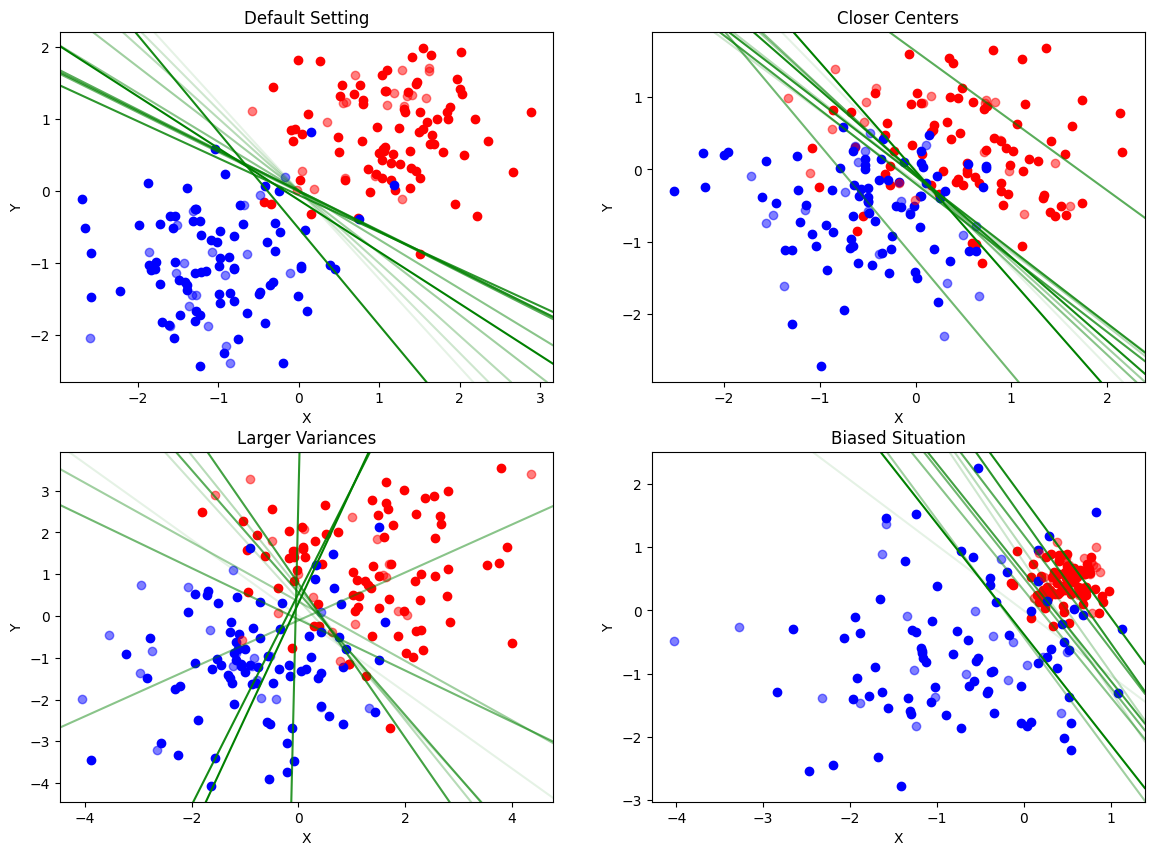
\includegraphics[width=0.5\linewidth]{fig_sec1_exp1.png}
    \caption{Perceptrons trained on Gaussian-distributed datasets.}
    \label{fig:sec1_exp1}
\end{figure}

\section{Multiple-layer Perceptron (MLP)}

\subsection{Mathematical model}

We still use the binary classification problem as an example, so the problem definition is the same.

\subsection{Machine learning model}

In order to classify the different samples more accurately, we want to replace lines and hyperplanes with need curves and hyper-surfaces. A MLP, including several hidden layers and a output layer, is what we need. This is because the family of neural networks is dense in the function space, known as the Universal Approximation Theorem\cite{uat}. A layer is formed with several parallel perceptrons, each takes all the output values of the last layer as the input. In MLP, perceptrons in hidden layers use ReLU as activation function and perceptrons in the output layer uses SoftMax since Max is non-differentiable.

Formally, let $L(L\geq 2)$ be the total number of layers, including both hidden layers and the output layer. Our model $W$ takes a vector $\mathbf{x}\in\mathbb{R}^d$ as input, and outputs a prediction vector $\hat{\mathbf{y}}\in[0,1]^m$, where $m$ is the number of classes. $\mathbf{W}^{(l)} \in \mathbb{R}^{n_l \times n_{l-1}}$ is the weight matrix of layer $l$, where $n_l$ is the number of neurons in layer $l$ and $n_{l-1}$ is the number of neurons in the previous layer. $\mathbf{b}^{(l)} \in \mathbb{R}^{n_l}$ is the bias vector of layer $l$. $\mathbf{z}^{(l)} \in \mathbb{R}^{n_l}$ is the linear combination of the inputs to layer $l$ before applying the activation function. $\mathbf{a}^{(l)} \in \mathbb{R}^{n_l}$ is the output of layer $l$ after applying the activation function. $n_0=d,n_L=m$.

\subsection{Forwarding}

For the first layer, $\mathbf{a}^{(0)} = \mathbf{x}$.

Each hidden layer $(1\le l < L)$ takes the output of the last layer as input,

$$
\mathbf{z}^{(l)} = \mathbf{W}^{(l)} \mathbf{a}^{(l-1)} + \mathbf{b}^{(l)}.
$$

Then the hidden layer uses ReLU as the activation function,

$$
\mathbf{a}^{(l)} = \text{ReLU}(\mathbf{z}^{(l)}) = \max(0, \mathbf{z}^{(l)}).
$$

The output layer takes the output of the last hidden layer as input,

$$
\mathbf{z}^{(L)} = \mathbf{W}^{(L)} \mathbf{a}^{(L-1)} + \mathbf{b}^{(L)}.
$$

Then the output layer uses SoftMax as the activation function,
$$
\mathbf{a}^{(L)}_i = \frac{e^{\mathbf{z}^{(L)}_i}}{\sum_{j=1}^{n_L} e^{\mathbf{z}^{(L)}_j}}.
$$

Finally, the output is $\hat{\mathbf{y}}=\mathbf{a}^{(L)}$.

\subsection{Loss function}

The CrossEntropy function is usually used as the loss function classification problems. The definition of the CrossEntropy function with input label $\mathbf{y} = [y_1, y_2, \dots, y_m]$ and prediction $\hat{\mathbf{y}} = [\hat{y}_1, \hat{y}_2, \dots, \hat{y}_m]$ is

$$
\mathcal{L} = -\sum_{i=1}^{m} y_i \log(\hat{y}_i),
$$ where $\mathbf{y}$ is the one-hot encoding of the label $y$.

\subsection{Backwarding}

Now we need to calculate the gradient of the weights of each component in the MLP with respect to the output of that component. Specially, the gradient of the SoftMax function and the gradient of the CrossEntropy function are always combined in practice for convenience.

\subsubsection{Output layer and CrossEntropy}

The gradient of the CrossEntropy function with respect to each $\hat{y}_i$ is

$$
\frac{\partial \mathcal{L}}{\partial \hat{y}_i} = \frac{\partial}{\partial \hat{y}_i}(-\sum_{j=1}^{m} y_j \log(\hat{y}_j)) = -\frac{y_i}{\hat{y}_i}
$$

To calculate the gradient of the output of the SoftMax with respect to its input, we need to calculate the gradient of each $\hat{y}_i$ with respect to each $z_j$.

When $i = j$,

$$
\frac{\partial \hat{y}_i}{\partial z_i}
= \frac{\partial}{\partial z_i} \left( \frac{e^{z_i}}{\sum_{j} e^{z_j}} \right)
= \frac{\sum_{j} e^{z_j} \cdot e^{z_i} - e^{z_i} \cdot e^{z_i}}{\left( \sum_{j} e^{z_j} \right)^2}
= \frac{e^{z_i}}{\sum_{j} e^{z_j}} \left( 1 - \frac{e^{z_i}}{\sum_{j} e^{z_j}} \right)
= \hat{y}_i (1 - \hat{y}_i),
$$

and when $i \neq j$,

$$
\frac{\partial \hat{y}_i}{\partial z_j}
= \frac{\partial}{\partial z_j} \left( \frac{e^{z_i}}{\sum_{k} e^{z_k}} \right)\\
= 0 - \frac{e^{z_i} \cdot e^{z_j}}{\left( \sum_{k} e^{z_k} \right)^2}\\
= - \hat{y}_i \hat{y}_j.
$$

Finally,

$$
\frac{\partial \mathcal{L}}{\partial z_j}
= -\sum_i y_i \frac{1}{\hat{y}_i} \frac{\partial \hat{y}_i}{\partial z_j}\\
= -y_j (1 - \hat{y}_j) + \sum_{i \neq j} y_i \hat{y}_j\\
= (\sum_i y_i)\hat{y}_j - y_j\\
= \hat{y}_j - y_j.
$$

Therefore,

$$
\delta^{(L)} = \frac{\partial \mathcal{L}}{\partial \mathbf{z}^{(L)}} = \mathbf{a}^{(L)} - \mathbf{y},
$$ and for the linear layer,

$$
\frac{\partial \mathcal{L}}{\partial \mathbf{W}^{(L)}} = \delta^{(L)} \mathbf{a}^{(L-1)T}, \frac{\partial \mathcal{L}}{\partial \mathbf{b}^{(L)}} = \delta^{(L)}.
$$

\subsubsection{Hidden layers}

The gradient of the activation function ReLU's output with respect to its input is obvious,

$$
\frac{\partial a^{(l)}}{\partial z^{(l)}} = \frac{\partial}{\partial z^{(l)}}\text{ReLU}(z^{(l)}) = I(z^{(l)} > 0).
$$

Therefore,

$$
\delta^{(l)} = \frac{\partial \mathcal{L}}{\partial \mathbf{z}^{(l)}}
= \frac{\partial \mathcal{L}}{\partial \mathbf{z}^{(l+1)}}
\frac{\partial \mathbf{z}^{(l+1)}}{\partial \mathbf{a}^{(l)}}
\frac{\partial \mathbf{a}^{(l)}}{\partial \mathbf{z}^{(l)}}
= (W^{(l+1)T} \delta^{(l+1)}) \odot I(z^{(l)} > 0),
$$ and for the linear layer,

$$
\frac{\partial \mathcal{L}}{\partial \mathbf{W}^{(l)}} = \delta^{(l)} \mathbf{a}^{(l-1)T}, \frac{\partial \mathcal{L}}{\partial \mathbf{b}^{(l)}} = \delta^{(l)}.
$$

\subsection{Gradient descent}

The weights and biases are updated using the gradient,

$$
\mathbf{W}^{(l)} \leftarrow \mathbf{W}^{(l)} - \eta \times \frac{\partial \mathcal{L}}{\partial \mathbf{W}^{(l)}},
$$

$$
\mathbf{b}^{(l)} \leftarrow \mathbf{b}^{(l)} - \eta \times \frac{\partial \mathcal{L}}{\partial \mathbf{b}^{(l)}},
$$ where $\eta$ is the learning rate.

\subsection{Experiment}

In the assignment, we test the MLP on a moon-like dataset generated by make\_moons method in sklearn, and record the loss and accuracy curve in \cref{fig:sec2_exp1}. The MLP has one hidden layer with $20$ units. The loss gently decreases, while the accuracy has clear plateaus and steep increases.

\begin{figure}
    \centering
    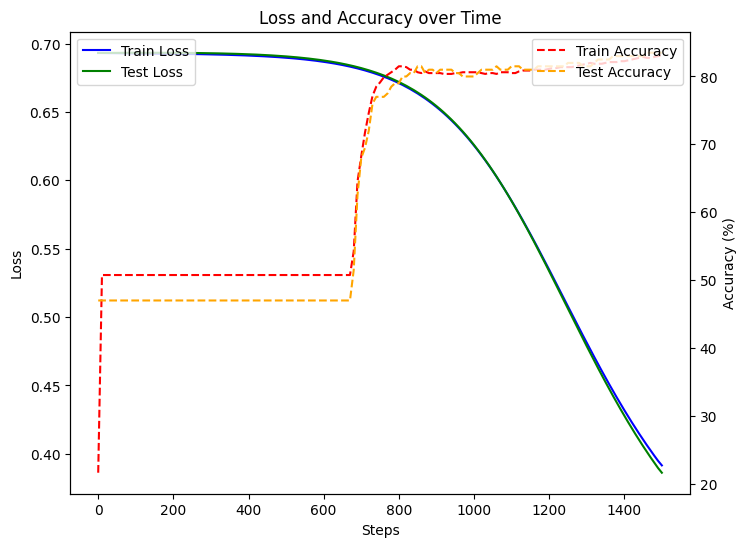
\includegraphics[width=0.5\linewidth]{fig_sec2_exp1.png}
    \caption{Loss and Accuracy over Time}
    \label{fig:sec2_exp1}
\end{figure}

\section{Stochastic Gradient Descent}

\begin{figure}[tb]
    \centering
    \begin{subfigure}{0.3\textwidth}
        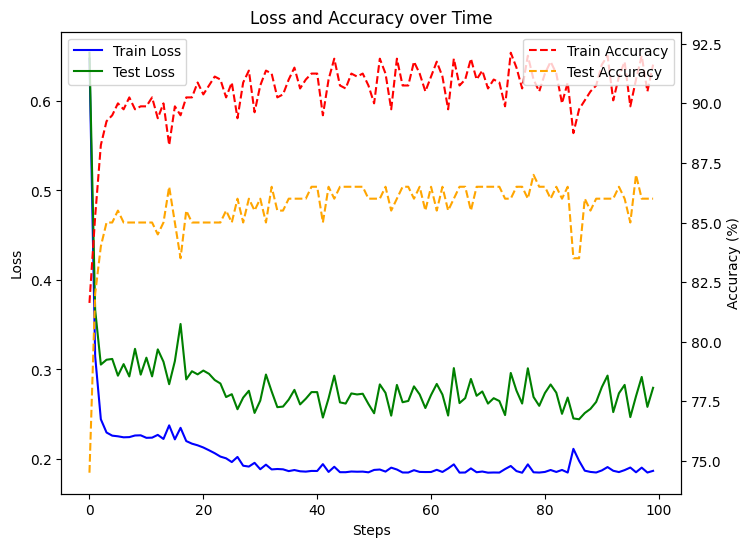
\includegraphics[width=\linewidth]{fig_sec3_exp1.png}
        \caption{$\text{Batch-size}=1$}
    \end{subfigure}
    \begin{subfigure}{0.3\textwidth}
        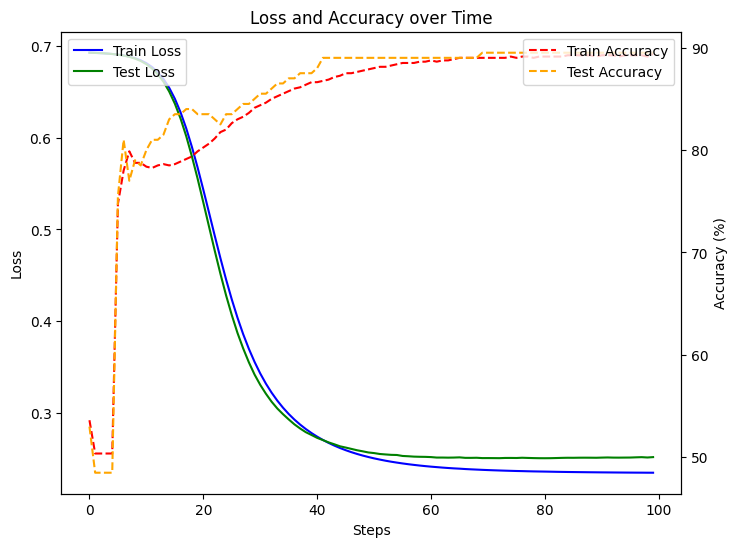
\includegraphics[width=\linewidth]{fig_sec3_exp2.png}
        \caption{$\text{Batch-size}=16$}
    \end{subfigure}
    \begin{subfigure}{0.3\textwidth}
        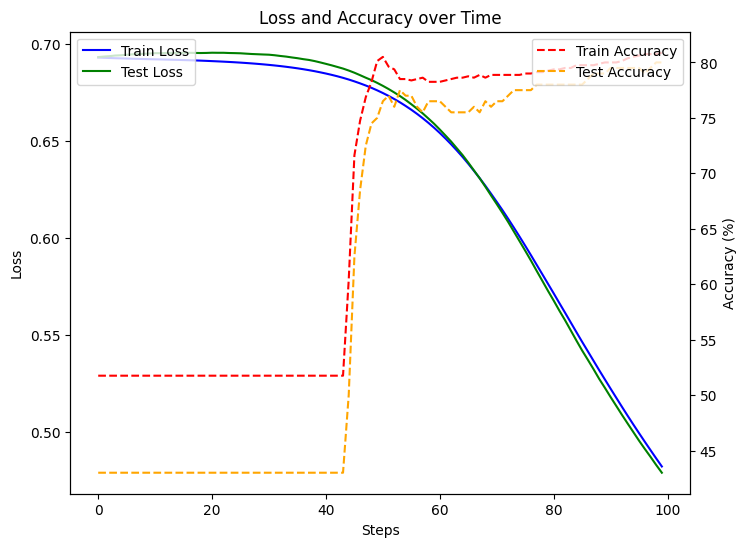
\includegraphics[width=\linewidth]{fig_sec3_exp3.png}
        \caption{$\text{Batch-size}=64$}
    \end{subfigure}
    \caption{Loss and Accuracy over Time with Different Batch-sizes.}
    \label{fig:sec3_exp123}
\end{figure}

While the vanilla gradient descent uses the average gradient of the entire training set for each epoch, the Stochastic Gradient Descent (SGD) calculates the gradient for each epoch using a random small batch of samples.

The main advantages of SGD include high computational efficiency, fast convergence speed, and the ability to escape local optima. SGD is typically more practical and effective for large-scale datasets and deep-learning tasks than vanilla gradient descent.

Here we test the MLP used in the last section with different batch-sizes, see \cref{fig:sec3_exp123}. $\text{Batch-size}=1$ achieves the highest train accuracy but slightly lower test accuracy, with very unstable loss curves. $\text{Batch-size}=16$ achieves both good train accuracy and good test accuracy, and smooth loss curves. $\text{Batch-size}=64$ shows smooth loss curves but learns slowly. Therefore an appropriate batch-size is important.

We can also see SGD's ability to escape local optima by testing with a MLP with two hidden layers in \cref{fig:sec3_exp2_12}. Without the SGD, a deeper MLP always overfits.

\begin{figure}[tb]
    \centering
    \begin{subfigure}{0.45\textwidth}
        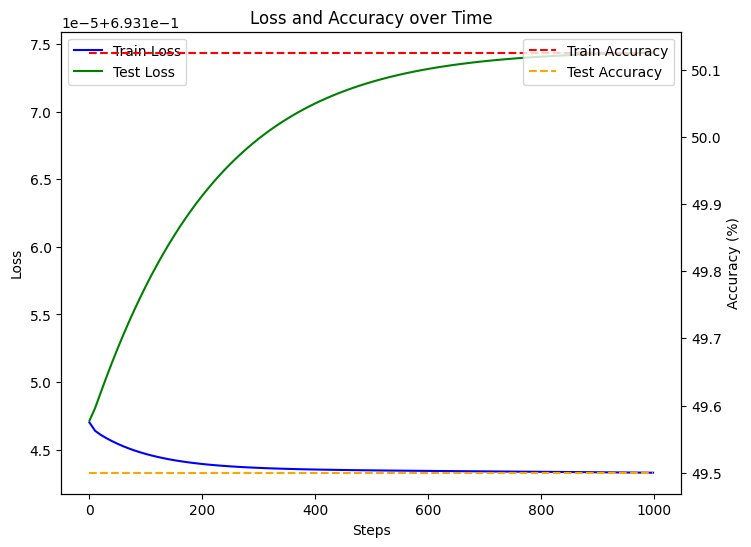
\includegraphics[width=\linewidth]{fig_sec3_exp2_1.png}
        \caption{Vanilla Gradient Descent}
    \end{subfigure}
    \begin{subfigure}{0.45\textwidth}
        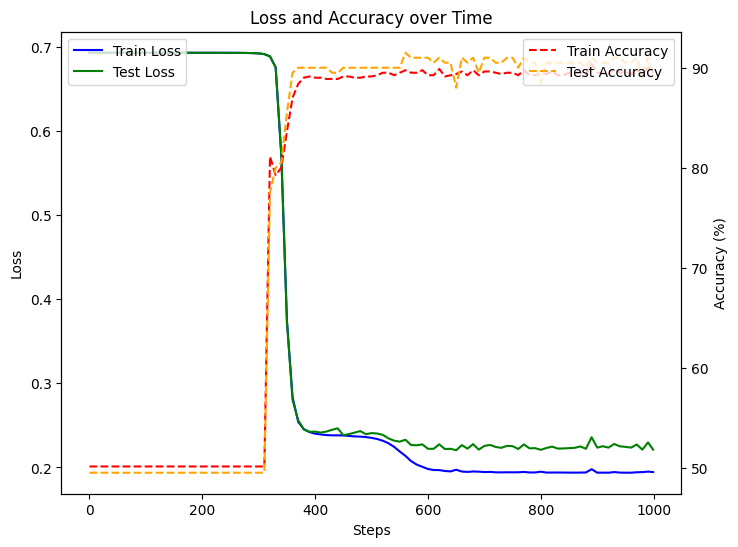
\includegraphics[width=\linewidth]{fig_sec3_exp2_2.png}
        \caption{Stochastic Gradient Descent}
    \end{subfigure}
    \caption{Deeper MLP with and without SGD.}
    \label{fig:sec3_exp2_12}
\end{figure}

\bibliographystyle{plain}
\bibliography{main}

% --------------------------------------------------------------
%     You don't have to mess with anything below this line.
% --------------------------------------------------------------
 
\end{document}
